\section{Dimensionless Analysis and Matched-Velocity Invariance}
\label{sec:analysis}

\subsection{One-period rest-to-rest reachability}

Translate the initial position to zero and consider positive displacement; the negative case follows by sign reversal. The terminal conditions are
\begin{equation}
 p(0)=0,quad v(0)=a(0)=0,qquad v(T)=a(T)=0.
 \label{eq:rest-boundary-conditions}
\end{equation}
We first exclude an active velocity bound and return to its sufficient condition in the theorem statement.

\begin{theorem}[One-period rest-to-rest displacement]
\label{thm:rest-boundary}
For the system in \cref{eq:third-order,eq:bounds} with the boundary conditions in \cref{eq:rest-boundary-conditions}, suppose the position is unconstrained and $V\ge2\vcrit$. The maximum reachable absolute displacement in duration $T$ is
\begin{equation}
 \dcrit=T\vcrit,
 \qquad
 \vcrit=
 \begin{cases}
 \displaystyle \frac{JT^2}{32}, & A\ge \dfrac{JT}{4},\\[6pt]
 \displaystyle \frac{AT}{4}-\frac{A^2}{2J}, & A<\dfrac{JT}{4}.
 \end{cases}
 \label{eq:vcrit}
\end{equation}
Every displacement $d$ satisfying $\abs d\le\dcrit$ is reachable with $v(T)=a(T)=0$.
\end{theorem}

\begin{proof}[Proof sketch]
The reachable set at fixed $T$ is convex and the terminal displacement is a linear functional of the jerk. Pontryagin's maximum principle, including acceleration-boundary arcs, therefore places an extremizer at $j\in\{-J,0,J\}$ with $a\in\{-A,A\}$ whenever the corresponding state bound is active~\cite{pontryagin1962maximum}. Time reversal and sign reflection give an extremal acceleration that is nonnegative on the first half, nonpositive on the second, and antisymmetric about $T/2$. On $[0,T/2]$ its pointwise upper envelope is obtained by ramping from zero with $+J$, respecting $A$, and ramping back to zero with $-J$ in time to mirror the deceleration half.

If $A\ge JT/4$, the acceleration is triangular, with four equal jerk segments $+J,-J,-J,+J$ of duration $T/4$. The midpoint velocity is $JT^2/16$. If $A<JT/4$, let $h=A/J$; the first half contains a ramp of duration $h$, an acceleration plateau of duration $T/2-2h$, and a ramp down of duration $h$, yielding midpoint velocity $AT/2-A^2/J$. The optimal velocity profile is symmetric, and its integral is $T/2$ times the midpoint velocity, which gives \cref{eq:vcrit}. Thus the maximum speed on the profile is $2\vcrit$, explaining the sufficient condition on $V$. Scaling the signed jerk and resulting state by $\abs d/\dcrit$ constructs every smaller displacement. A complete upper-bound and segment-integration argument appears in \cref{app:proofs}.
\end{proof}

The theorem is a reachability result. It identifies a feasible extremal rest-to-rest transfer and proves that a larger one is impossible under the stated assumptions. It does not specify which feasible profile an arbitrary OTG selects, nor does it cover an active velocity limit, asymmetric bounds, position constraints, plant dynamics, or multiple synchronized axes.

\subsection{Dimensionless boundary}

Substituting $q=4A/(JT)$ into \cref{eq:vcrit} gives
\begin{equation}
 \frac{\vcrit}{JT^2}=g(q)=
 \begin{cases}
 \dfrac{2q-q^2}{32}, & 0<q<1,\\[4pt]
 \dfrac{1}{32}, & q\ge1.
 \end{cases}
 \label{eq:gq}
\end{equation}
The two branches and the E15 phase coordinates are shown in \cref{fig:dimensionless-boundary}. The function and its first derivative are continuous at $q=1$, while the active profile topology changes from acceleration-limited to jerk-limited.

\begin{figure*}[t]
 \centering
 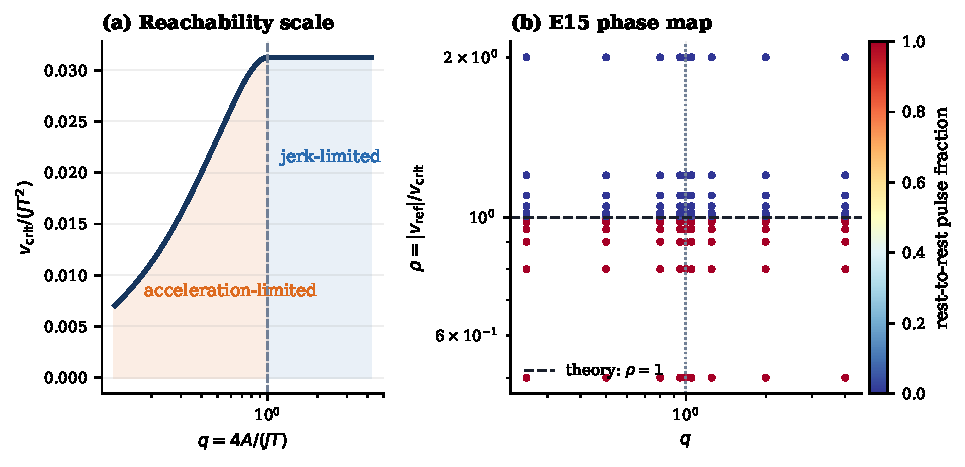
\includegraphics[width=\textwidth]{figures/generated/fig2_dimensionless_boundary.pdf}
 \caption{Dimensionless prediction. (a) The normalized critical speed has an acceleration-limited branch for $q<1$ and a saturated jerk-limited branch for $q\ge1$. (b) E15 configurations colored by observed rest-to-rest pulse fraction. The horizontal line $\rho=1$ is theoretical; the solver realization is empirical.}
 \label{fig:dimensionless-boundary}
\end{figure*}

\begin{corollary}[Dimensionless rest-to-rest boundary]
\label{cor:rho-boundary}
For the constant schedule in \cref{eq:constant-schedule}, a P-only transfer over one tick requires displacement $\abs{\vref}T$. Under the assumptions of \cref{thm:rest-boundary}, this transfer with terminal $v=a=0$ is reachable if and only if
\begin{equation}
 \rho=\frac{\abs{\vref}}{\vcrit}\le1.
 \label{eq:rho-boundary}
\end{equation}
\end{corollary}

If an OTG exactly completes that reachable P-only transfer and the next tick begins from its terminal rest state, repeated application produces a sequence of rest-to-rest pulses. That conditional statement explains the mechanism. The stronger statement that Ruckig~\RuckigVersion{} realizes this transition over the tested grid is established only by E15 in \cref{sec:boundary-results}. At the exact seam, numerical behavior is explicitly treated as diagnostic rather than absorbed into the theorem.\claimtag{C1}\claimtag{C2}

\begin{corollary}[Monotonic design implication]
\label{cor:monotonic}
For fixed values of the other quantities, $\vcrit$ is nondecreasing in $A$, $J$, and $T$. Hence increasing a limit or lengthening the control period weakly decreases $\rho$ for a fixed $\vref$ and can enlarge the one-period rest-to-rest region.
\end{corollary}

The dependence saturates in $A$ once $A\ge JT/4$, but it is otherwise strict. This is why limit tuning is not a reliable semantic repair: a seemingly more capable generator can become more capable of satisfying the unintended stop request.

\subsection{Matched-velocity continuation}

\begin{proposition}[Matched-PV invariant continuation]
\label{prop:matched-pv}
Suppose the current state lies on a constant-speed reference, $(p_k,\vref,0)$, with $\abs{\vref}\le V$. For target $(p_k+\vref T,\vref,0)$, the trajectory
\begin{equation}
 p(\tau)=p_k+\vref\tau,qquad
 v(\tau)=\vref,qquad a(\tau)=j(\tau)=0
 \label{eq:matched-continuation}
\end{equation}
for $0\le\tau\le T$ is feasible and exactly reaches the target.
\end{proposition}

\begin{proof}
Direct substitution satisfies the dynamics, endpoint state, and all acceleration and jerk bounds. The velocity bound follows from $\abs{\vref}\le V$.
\end{proof}

The proposition establishes existence, not solver preference or uniqueness under an unspecified objective. In E16, matched/oracle PV empirically reproduces this exact zero-ripple profile in every tested primary cell. In contrast, the P-only requirement $v(T)=0$ is structurally incompatible with \cref{eq:matched-continuation} whenever $\vref\ne0$.\claimtag{C3}

\begin{lemma}[Fixed-grid causality and affine exactness]
\label{lem:future-o1}
Under the information set in \cref{eq:information-set}, \FutureOOne{} in \cref{eq:future-o1} is causal. If $P[k]=c_0+c_1kT$, then $\widehat V[k+1]=c_1$ exactly.
\end{lemma}

\begin{proof}
The expression reads only samples with indices at most $k$. Substituting the affine sequence gives
$2(c_0+c_1kT)-3(c_0+c_1(k-1)T)+(c_0+c_1(k-2)T)=c_1T$.
\end{proof}

The lemma does not imply noise optimality, validity on an irregular grid, or superiority for arbitrary trajectories. Those are empirical questions, and the observer selected in the synthetic robustness experiment differs from the one selected for the recorded fixed-grid case.\claimtag{C5}

